\section{Probability of a Sequence}
\begin{frame}{Probability of a sequence}
    \begin{figure}
        \centering
        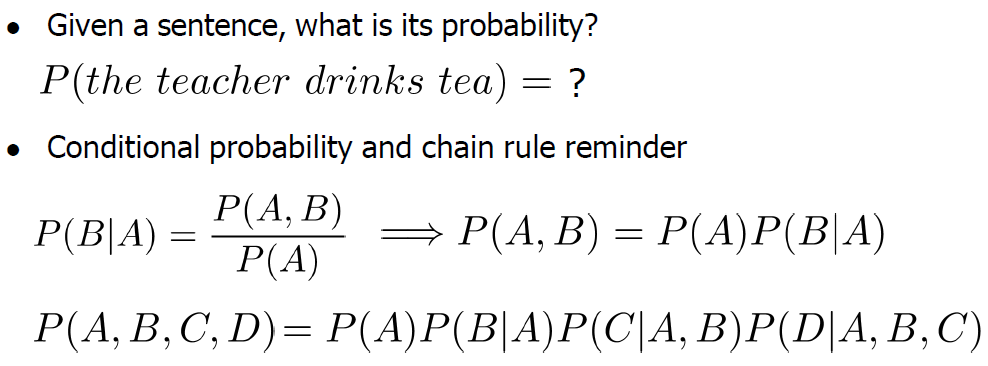
\includegraphics[width=\textwidth,height=0.8\textheight,keepaspectratio]{images/nlp-intro/prob-seq-1.png}
    \end{figure}
\end{frame}

\begin{frame}{Probability of a sequence}
    \begin{figure}
        \centering
        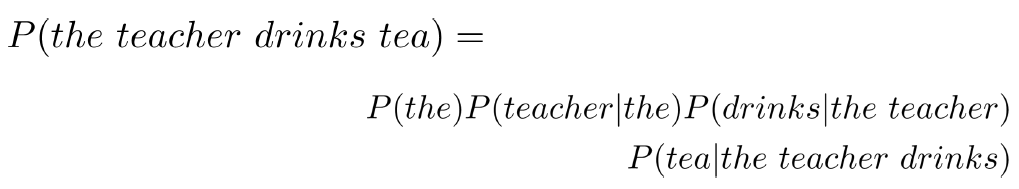
\includegraphics[width=\textwidth,height=0.8\textheight,keepaspectratio]{images/nlp-intro/prob-seq-2.png}
    \end{figure}
\end{frame}

\begin{frame}{Sentence not in corpus}
    \textbf{Problem:} Corpus almost never contains the exact sentence we’re interested in or even its longer subsequences! \\[1em]
    \begin{figure}
        \centering
        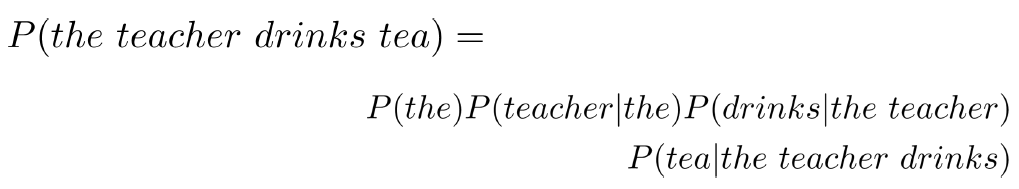
\includegraphics[width=\textwidth,height=0.7\textheight,keepaspectratio]{images/nlp-intro/prob-seq-2.png}
    \end{figure}
\end{frame}

\begin{frame}{Approximation of sequence probability}
    \begin{figure}
        \centering
        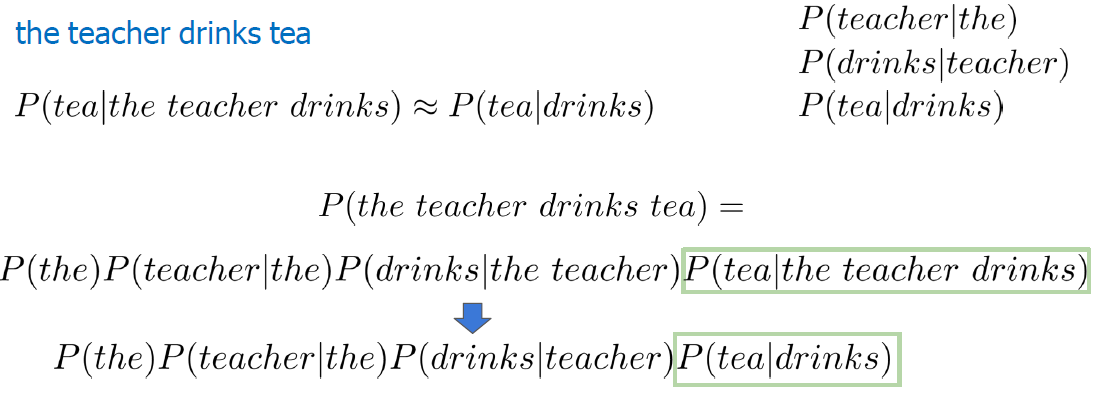
\includegraphics[width=\textwidth,height=0.8\textheight,keepaspectratio]{images/nlp-intro/approx-seq-prob.png}
    \end{figure}
\end{frame}

\begin{frame}{Approximation of sequence probability}
    \begin{figure}
        \centering
        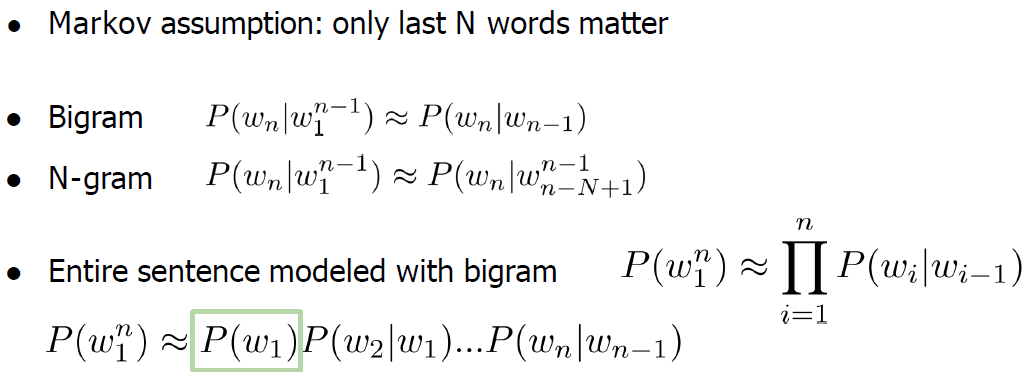
\includegraphics[width=\textwidth,height=0.8\textheight,keepaspectratio]{images/nlp-intro/approx-seq-prob-2.png}
    \end{figure}
\end{frame}

\begin{frame}{Quiz}
    \begin{figure}
        \centering
        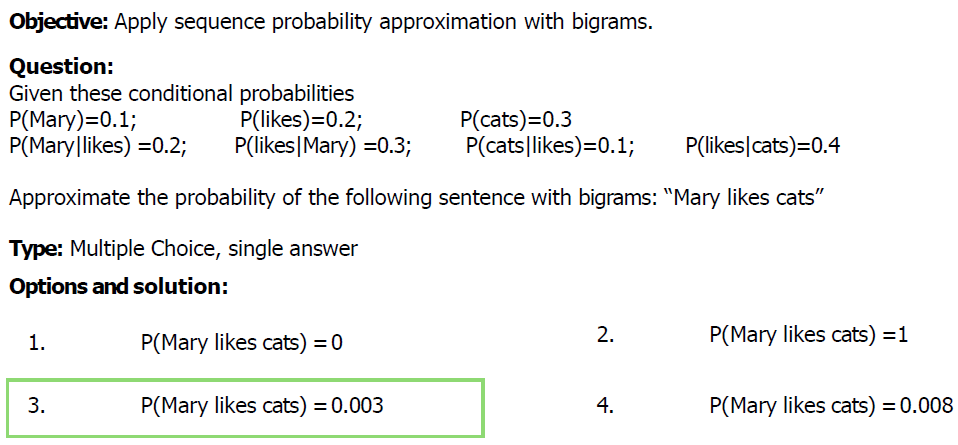
\includegraphics[width=\textwidth,height=0.8\textheight,keepaspectratio]{images/nlp-intro/quiz-seq-prob.png}
    \end{figure}
\end{frame}